\subsection{Registration}\label{subsec:chp3:img-reg:reg}
\begin{figure}
\centering

% Define block styles used later

\tikzstyle{module}=[draw, draw=blue!80, text width=10em,
    text centered, minimum height=5em, minimum width = 10em, drop shadow, rounded corners,
    fill=blue!30]

\tikzstyle{vecArrow} = [thick, decoration={markings,mark=at position
   1 with {\arrow[semithick]{open triangle 60}}},
   double distance=1.4pt, shorten >= 5.5pt,
   preaction = {decorate},
   postaction = {draw,line width=1.4pt, white,shorten >= 4.5pt}]

% Define distances for bordering
\def\blockdist{1.5}
\def\edgedist{2.5}

\definecolor{darkblue}{rgb}{0.2,0.2,0.6}
\definecolor{darkred}{rgb}{0.6,0.1,0.1}
\definecolor{darkgreen}{rgb}{0.2,0.6,0.2}

\def\arrow{
  (10.75:1.1) -- (6.5:1) arc (6.25:120:1) [rounded corners=0.5] --
  (120:0.9) [rounded corners=1] -- (130:1.1) [rounded corners=0.5] --
  (120:1.3) [sharp corners] -- (120:1.2) arc (120:5.25:1.2)
  [rounded corners=1] -- (10.75:1.1) -- (6.5:1) -- cycle
}

\tikzset{
  ashadow/.style={opacity=.25, shadow xshift=0.07, shadow yshift=-0.07},
}

\def\arrows[#1]{
  \begin{scope}[scale=#1]
	\node[align=center] at (0,0) {\Huge{ Loop } \\ \Huge{ until matching } };

    \draw[color=darkred, %
    drop shadow={ashadow, color=red!60!black}] \arrow;

    \draw[color=darkgreen, bottom color=green!60!black, top color=green!30, %
    drop shadow={ashadow, color=green!60!black}] [rotate=120] \arrow;

    \draw[color=darkblue, right color=blue!60, left color=blue!30, %
    drop shadow={ashadow, color=blue!60!black}] [rotate=240] \arrow;

    % to hide the green shadow
    \draw[color=darkred, left color=red!60, right color=red!30] \arrow;
  \end{scope}
}

%\begin{tikzpicture}[node distance=3cm,thick,path image/.style={
\begin{tikzpicture}[node distance=3cm,thick,scale=0.5, every node/.style={scale=0.5},path image/.style={
path picture={
\node at (path picture bounding box.center) {
\includegraphics[width=1cm]{#1}
};}}]
\tikzstyle{conefill} = [path image=,fill opacity=0.8]

\node (t2w) at (0,0)	{\includegraphics[width=1.5cm]{2_modality/figures/tikzimage/dce.eps}};
\begin{scope}[node distance=1.2cm]
\node[below of=t2w] (cap1) {\Large Fixed};
\end{scope}
\begin{scope}[node distance=6cm]
\node[below of=t2w] 	(dce) 			{\includegraphics[width=1.5cm]{2_modality/figures/tikzimage/t2.eps}};
\begin{scope}[node distance=1.2cm]
\node[below of=dce] (cap2) {\Large Moving};
\end{scope}
\end{scope}

\begin{scope}[node distance=5.5cm]
	\node[module,right of=t2w] (sim) {\Large Similarity \\ measure};
\end{scope}
\begin{scope}[node distance=3cm]
	\node[module,below of=sim] (int) {\Large Interpolator};
	\node[module,below of=int] (tra) {\Large Transform};
\end{scope}

\draw[line width=1mm,draw=blue!30,->] (t2w)--(sim);
\draw[line width=1mm,draw=blue!30,->] (dce)--(tra);

\begin{scope}[node distance=9cm]
	\node[module,right of=sim] (opt) {\Large Optimizer};
\end{scope}

\draw[draw=blue,->,line width=.5mm] (tra)--(int);
\draw[draw=blue,->,line width=.5mm] (int)--(sim);
\draw[draw=blue,->,line width=.5mm] (sim)--(opt) node[midway,above] {\Large Similarity} node[midway,below] {\Large metric};
\draw[draw=blue,->,line width=.5mm] (opt)|-(tra);

\begin{pgfonlayer}{background}
	\path (sim.west |- sim.north)+(-0.5,.5) node (a) {};
    \path (opt.east |- tra.south)+(+0.5,-0.5) node (b) {};

    \path[fill=blue!10,rounded corners, draw=blue!20, dashed] (a) rectangle (b);
\end{pgfonlayer}

\begin{scope}[node distance=5cm]
\node[right of=int] (arr) {
\begin{tikzpicture}
\arrows[1.9];
\end{tikzpicture}
};
\end{scope}
\end{tikzpicture}
\caption[Registration framework.]{Typical framework involved to solve the registration problem.}
\label{fig:frareg}
\end{figure}



%\tikzset{
%  ashadow/.style={opacity=.25, shadow xshift=0.07, shadow yshift=-0.07},
%}
%
%\def\arrows[#1]{
%  \begin{scope}[scale=#1]
%	\node[align=center] at (0,0) {Loop \\ until \\ matching};
%
%    \draw[color=darkred, %
%    drop shadow={ashadow, color=red!60!black}] \arrow;
%
%    \draw[color=darkgreen, bottom color=green!60!black, top color=green!30, %
%    drop shadow={ashadow, color=green!60!black}] [rotate=120] \arrow;
%
%    \draw[color=darkblue, right color=blue!60, left color=blue!30, %
%    drop shadow={ashadow, color=blue!60!black}] [rotate=240] \arrow;
%
%    % to hide the green shadow
%    \draw[color=darkred, left color=red!60, right color=red!30] \arrow;
%  \end{scope}
%}
%
%\begin{tikzpicture}[node distance=3cm,thick,path image/.style={
%path picture={
%\node at (path picture bounding box.center) {
%\includegraphics[width=.5cm]{#1}
%};}}]
%\tikzstyle{conefill} = [path image=,fill opacity=0.8]
%
%\node[inner sep=0pt] (t2w) at (0,0)	{\includegraphics[width=1cm]{02_background/figures/tikzimage/dce.eps}};
%\begin{scope}[node distance=.8cm]
%\node[below of=t2w] (cap1) {Fixed};
%\end{scope}
%\begin{scope}[node distance=3.5cm]
%\node[below of=t2w] 	(dce) 			{\includegraphics[width=1cm]{02_background/figures/tikzimage/t2.eps}};
%\begin{scope}[node distance=.8cm]
%\node[below of=dce] (cap2) {Moving};
%\end{scope}
%\end{scope}
%
%\begin{scope}[node distance=2.5cm]
%	\node[module,right of=t2w] (sim) {Similarity \\ measure};
%\end{scope}
%\begin{scope}[node distance=1.75cm]
%	\node[module,below of=sim] (int) {Interpolator};
%	\node[module,below of=int] (tra) {Transform};
%\end{scope}
%\begin{scope}[node distance=5cm]
%	\node[module,right of=sim] (opt) {Optimizer};
%\end{scope}
%
%\draw[draw=blue,->,line width=.5mm] (tra)--(int);
%\draw[draw=blue,->,line width=.5mm] (int)--(sim);
%\draw[draw=blue,->,line width=.5mm] (sim)--(opt) node[midway,above] {Similarity} node[midway,below] {metric};
%\draw[draw=blue,->,line width=.5mm] (opt)|-(tra);
%
%\draw[line width=.8mm,draw=blue!30,->] (t2w)--(sim);
%\draw[line width=.8mm,draw=blue!30,->] (dce)--(tra);
%
%\begin{pgfonlayer}{background}
%	\path (sim.west |- sim.north)+(-0.3,.3) node (a) {};
%    \path (opt.east |- tra.south)+(+0.3,-0.3) node (b) {};
%
%    \path[fill=blue!10,rounded corners, draw=blue!20, dashed] (a) rectangle (b);
%\end{pgfonlayer}
%
%\begin{scope}[node distance=3cm]
%\node[right of=int] (arr) {
%\begin{tikzpicture}
%\arrows[1];
%\end{tikzpicture}
%};
%\end{scope}


Image registration plays a vital role in \ac{cad} systems using \ac{mpmri}
images.
As it will be discussed in \acs{sec}\,\ref{sec:chp3:img-clas}, the features
detected in each modality are grouped depending of their spatial location,
requiring a perfect alignment of the \ac{mpmri} ahead of the classification.

Image registration is the procedure consisting of aligning an unregistered
image --- also called moving image --- into a template image --- also called
fixed image --- via a geometric transformation.
This problem is usually addressed as depicted in \ac{fig}\,\ref{fig:frareg}.
An iterative procedure takes place to infer the geometric transformation,
parametric or non-parametric, via an optimizer which maximizes the similarity
between the two images.
In the following, a review of the different components of a typical
registration framework: transformation model, similarity metric, optimizer, and
interpolation are presented.
To conclude a summary is given focusing on the registration approaches applied in \ac{cad} for \ac{cap} systems.
Exhaustive reviews covering all registration methods in computer science and
medical fields can be found in~\cite{Maintz1998,Zitova2003}.

\setenumerate{listparindent=\parindent,itemsep=10px}
\setlist{noitemsep}
\begin{enumerate}[leftmargin=*]

\item[] \textbf{Geometric transformation models}
As previously mentioned, the registration process is equivalent to find a
geometric transformation which minimizes the difference between two images.
From all \ac{cad} systems reviewed, only parametric methods have been
implemented.
Three different groups of parametric transformation models have been used ---
i.e., rigid, affine, and elastic --- each of them characterized by a specific
degree of freedom.

The simplest transformation used in terms of degrees of freedom is usually
referred to as rigid transformation.
This type of transformation is only composed of a rotation and a translation.
Therefore, for the 2D case where $\mathbf{x} = (x,y) \in \mathbb{R}^2$, a rigid
transformation $\mathcal{T}_R$ is formalized as:

\begin{eqnarray}
  \mathcal{T}_R(\mathbf{x}) & = & \begin{bmatrix}
    R & \mathbf{t} \\
    \mathbf{0^T} & 1
  \end{bmatrix} \mathbf{x} \ , \nonumber \\
                            & = & \begin{bmatrix}
                              \cos \theta & -\sin \theta & t_x \\
                              \sin \theta & \cos \theta & t_y \\
                              0 & 0 & 1
                            \end{bmatrix}\begin{bmatrix}
                              x \\
                              y \\
                              1
                            \end{bmatrix} \ , \label{eq:rigtra} %\\
\end{eqnarray}

\noindent where $\theta$ is the rotation angle and $\{ t_x,t_y \}$ represents
the translation along $\{x,y\}$ respectively.
In the case of 3D registration using volume, an additional component $z$ is
introduced such that $\mathbf{x} = (x,y,z)$.
Thus, the rotation matrix $\mathbf{R}$ becomes of size $3 \times 3$ whereas the
translation vector $\mathbf{t}$ consists of a vector of 3 variables.
The geometric transformation $\mathcal{T}_R(\cdot)$ is embedded into a matrix
of size $4 \times 4$.

The affine transformation provides additional degrees of freedom, providing
rotation, translation, --- as with the rigid transformations --- and also
shearing and scaling.
Hence, for a 2D space where $\mathbf{x} = (x,y) \in \mathbb{R}^2$, an affine
transformation $\mathcal{T}_A$ is formalized as:

\begin{eqnarray}
  \mathcal{T}_A(\mathbf{x}) & = & \begin{bmatrix}
    A & \mathbf{t} \\
    \mathbf{0^T} & 1
  \end{bmatrix} \mathbf{x} \ , \nonumber \\
                            & = & \begin{bmatrix}
                              a_{11} & a_{12} & t_x \\
                              a_{21} & a_{22} & t_y \\
                              0 & 0 & 1
                            \end{bmatrix}\begin{bmatrix}
                              x \\
                              y \\
                              1
                            \end{bmatrix} \ . \label{eq:afftra}%
\end{eqnarray}

\noindent where the 4 parameters $\{a_{11},a_{12},a_{21},a_{22}\}$ of the
affine matrix and $\{ t_x, t_y \}$ of the translation encode the deformation.
As in the rigid registration case, in 3D the affine transformation
$\mathcal{T}_A(\cdot)$ is of size $4 \times 4$ but now with 12 parameters
involved.

Finally, the last group of transformations is known as elastic transformations
and offers the advantage to handle local distortions.
In the reviewed \ac{cad} systems, the radial basis functions are used to
formalize the local distortions such as:

\begin{equation}
  \mathcal{T}_E(\mathbf{x}) = \begin{matrix}
    a_{11} x - a_{12} y + t_x + \sum_i c_i g(\| \mathbf{x} - p_i \|) \\
    a_{21} x + a_{22} y + t_y + \sum_i c_i g(\| \mathbf{x} - p_i \|)
  \end{matrix} \ ,
\end{equation}

\noindent where $\mathbf{x}$ are the control points in both images and
$g(\cdots)$ is the actual radial basis function.

Two radial basis functions are used: (i) the \ac{tps} and (ii) the B-splines.
Apart from the formalism, these two approaches have a main difference: with
B-splines, the control points are usually uniformly and densely placed on a
grid whereas with \ac{tps}, the control points correspond to some detected or
selected key points.
By using \ac{tps}, \citeauthor{Mitra2011} obtained more accurate and time
efficient results than with the B-splines strategy~\cite{Mitra2012a}.

It is reasonable to point out that usually only rigid or affine registrations
are used to register \ac{mpmri} from a same protocol.
Elastic registration methods are more commonly used to register multi-protocol
images such as histopathology with \ac{mri} images~\cite{Toth2008,Toth2009}.

\item[] \textbf{Similarity measure}
The most naive similarity measure used in reviewed registration framework is
the \acf{mse} of the \ac{si} of \ac{mri} images.
For a pair of images $I$ and $J$, the \ac{mse} is formalized as:

\begin{equation}
  \text{MSE} =\frac{1}{N} \sum_x \sum_y \left[ I(x,y) - J(x,y) \right]^2 \ ,
  \label{eq:mse}
\end{equation}

\noindent where $N$ is the total number of pixels.
This metric is not well suited when \ac{mpmri} images are involved due to the
tissue appearance variations between the different modalities.

\begin{figure}
  \centering
  \hspace*{\fill}
  \subfloat[Illustration of a joint histogram between two aligned
  image.]{\label{subfig:histoalgn}
\includegraphics[width=0.2\textwidth]{3_review/figures/processing/registration/histogram/jointhistoalg.eps}}
  \hfill
  \subfloat[Illustration of a joint histogram between two misaligned
  image.]{\label{subfig:histomisalgn}
    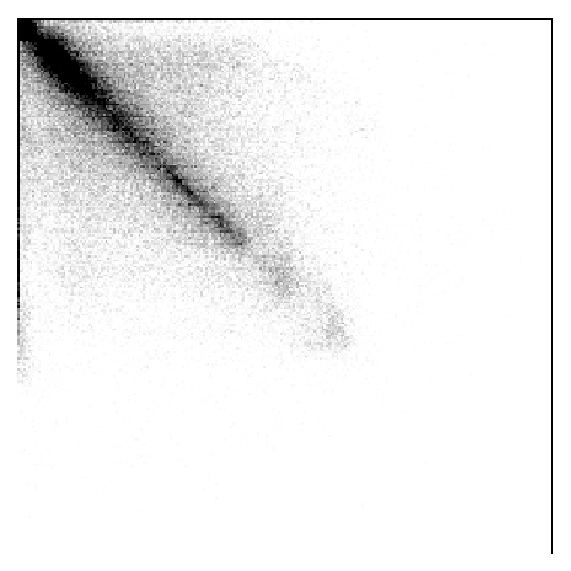
\includegraphics[width=0.2\textwidth]{3_review/figures/processing/registration/histogram/jointhistomisal.eps}}
  \hspace*{\fill}
  \caption[Difference observed in joint histogram between aligned and
  misaligned images.]{Difference observed in joint histogram between aligned
    and misaligned images. The joint measure will be more concentrated of the
    histogram in the case that the images are aligned and more randomly
    distributed in the case that both images are more misaligned.}
  \label{fig:jointhisto}
\end{figure}

In this regard, \ac{mi} was introduced as a similarity measure in registration
framework in the late 1990's by \citeauthor{Pluim2003}~\cite{Pluim2003}.
The \ac{mi} measure finds its foundation in the assumption that a homogeneous
region in the first modality image should also appear as a homogeneous region
in the second modality, even if their \acp{si} are not identical.
Thus, those regions share information and the registration task is achieved by
maximizing this common information.
Hence, \Ac{mi} of two images $A$ and $B$ is defined as:

\begin{equation}
  MI(A;B) = S(A) + S(B) - S(A,B) \ ,
  \label{eq:midef}
\end{equation}

\noindent where $S(A)$, $S(B)$, and $S(A,B)$ are the marginal entropies of $A$
and $B$ and the joint entropy, respectively.
Therefore, maximizing the \ac{mi} is the equivalent of minimizing the joint
entropy.
The joint entropy measure is related to the degree of uncertainty or dispersion
of the data in the joint histogram of the images $A$ and $B$.
As shown in \acs{fig}\,\ref{fig:jointhisto}, the data in the joint histogram
are concentrated in the case of aligned images (see
\acs{fig}\,\ref{subfig:histoalgn}) while it is more randomly distributed in the
case of misaligned images (see \acs{fig}\,\ref{subfig:histomisalgn}).
The entropy is computed based on an estimation of the \ac{pdf} of the images
and thus histogram or Parzen window methods are a common way to estimate these
\acp{pdf}.

A generalized form of \ac{mi}, \ac{cmi}, has been proposed by
\citeauthor{Chappelow2011}~\cite{Chappelow2011}.
\ac{cmi} encompasses interdependent information such as texture and gradient
information into the metric.
Hence, for both of images $A$ and $B$, the image ensembles $\epsilon^{A}_n$ and
$\epsilon^{B}_m$ are generated and composed of $n$ and $m$ images based on the
texture and gradient.
Then, the \ac{cmi} is formulated such as:

\begin{equation}
  CMI(\epsilon^{A}_n;\epsilon^{B}_m) = S(\epsilon^{A}_n) + S(\epsilon^{B}_m) -
  S(\epsilon^{A}_n,\epsilon^{B}_m) \ .
  \label{eq:cmidef}
\end{equation}

From \acs{eq}\,\eqref{eq:cmidef}, note that \ac{cmi} is estimated from
high-dimensional data and as a consequence the histogram-based methods to
estimate the \acp{pdf} are not suitable anymore~\cite{Chappelow2011}.
However, other alternative approaches are used such as the one employed
in~\cite{Staring2009} to compute the $\alpha$-\ac{mi}~\cite{Hero2002}.

\item[] \textbf{Optimization methods}
Registration is usually regarded as an optimization problem where the
parameters of the geometric transformation model have to be inferred by
minimizing/maximizing the similarity measure.
Iterative optimization methods are commonly used, where the most common methods
used are the L-BFGS-B quasi-Newton method~\cite{Byrd1995} and the gradient
descent~\cite{Viola1997}.
During our review, we noticed that authors do not usually linger over optimizer
choice.

\item[] \textbf{Interpolation}
The registration procedure involves transforming an image and pixels mapped to
non-integer points must be approximated using interpolation methods.
As for the optimization methods, we notice that little attention has been paid
on the choice of those interpolations methods.
However, commonly used methods are bi-linear, nearest-neighbour, bi-cubic,
spline, and inverse-distance weighting method~\cite{Mitra2012}.

\item[] \textbf{Registration methods used in \ac{cad} systems}
\acs{tab}~\ref{tab:regtab} summarizes the framework used to register \ac{mpmri}
images in \ac{cad} for \ac{cap}.

\begin{table}
  \centering
  \caption[Classification of the different registration methods used in the
  \acs*{cad} systems reviewed.]{Classification of the different registration
    methods used in the \acs*{cad} systems reviewed. Acronyms: mean squared
    error (MSE), mutual information (MI), combined mutual information (CMI),
    gradient descent (GD), limited-memory Broyden-Fletcher-Goldfarb-Shannon box
    constraints (L-BFGS-B).}
  \scriptsize
  \begin{threeparttable}
    \begin{tabular}{l l c c c c c c c c}\hline
      \toprule
      \textbf{Study} & \textbf{Modality} & \multirow{2}{*}{\textbf{Type}} &
                                                                            \multicolumn{2}{c}{\textbf{Geometric
                                                                            model}}
      & \multicolumn{3}{c}{\textbf{Similarity measure}} &
                                                          \multicolumn{2}{c}{\textbf{Optimizer}}
      \\
      \cmidrule(lr){4-5} \cmidrule(lr){6-8} \cmidrule(lr){9-10}
      \textbf{index} & \textbf{registered} & & Affine & Elastic & \acs{mse} &
                                                                              \acs{mi}
                                           & \acs{cmi} & GD & L-BFGS-B \\
      \midrule
      \cite{Ampeliotis2007,Ampeliotis2008} & \ac{t2w} - \ac{dce} & 2D & \cmark
      & $-$ & \cmark & $-$ & $-$ & $-$ & $-$ \\
      \cite{Giannini2013,giannini2015fully} & \ac{t2w} - \ac{dw} & 2D & \cmark
      & \cmark & $-$ & $-$ & $-$ & $-$ & $-$  \\
      \cite{Giannini2013,giannini2015fully} & \ac{t2w} - \ac{dce} & 2D & \cmark
      & \cmark & $-$ & \cmark & $-$ & \cmark & $-$ \\
      \cite{Viswanath2008a,Viswanath2009} & \ac{t2w} - \ac{dce} & 2D & \cmark &
                                                                                $-$
                                                        & $-$ & \cmark & $-$ &
                                                                               $-$ & $-$ \\
      \cite{Viswanath2011} & \ac{t2w} - \ac{dce} - \ac{dw} & 3D & \cmark & $-$
                                                        & $-$ & $-$ & \cmark &
                                                                               \cmark
                                                      & $-$  \\
      \cite{Vos2008} & \ac{t2w} - \ac{dce} & 3D & \cmark & $-$ & $-$ & \cmark &
                                                                                $-$
                                             & $-$ & $-$ \\
      \cite{Vos2010} & \ac{t2w} - \ac{dce} & 3D & \cmark & \cmark & $-$ &
                                                                          \cmark
                                           & $-$ & $-$ & \cmark \\
      \cite{Lemaitre2016thesis} & \ac{t2w} - \ac{dce} - \ac{dw} & 3D & \cmark & \cmark
                                                        & \cmark & \cmark & $-$ &
                                                                               \cmark
                                                      & $-$  \\
      \bottomrule
    \end{tabular}
    \begin{tablenotes}
      \footnotesize
    \item Notes:
    \item {$-$}: not used or not mentioned.
    \item {\cmark}: used or implemented.
    \end{tablenotes}
  \end{threeparttable}
  \label{tab:regtab}
\end{table}

\citeauthor{Ampeliotis2008} in~\cite{Ampeliotis2007,Ampeliotis2008} did not use
the framework as presented in \acs{fig}\,\ref{fig:frareg} to register 2D
\ac{t2w}-\ac{mri} and \ac{dce}-\ac{mri} images.
By using image symmetries and the \ac{mse} metric, they found the parameters of
an affine transformation but without using a common objective function.
The scale factor, the rotation, and the translation are independently and
sequentially estimated.

\citeauthor{Giannini2013} used also a in-house registration method for 2D
\ac{t2w}-\ac{mri} and \ac{dw}-\ac{mri} images using an affine
model~\cite{Giannini2013,giannini2015fully}.
The bladder is first segmented in both modalities in order to obtain its
contours which are then used as a metric function (i.e. distance between
contours) for registration.

\citeauthor{Giannini2013} and also \citeauthor{Vos2010} used a framework based
on finding an affine transformation to register the \ac{t2w}-\ac{mri} and
\ac{dce}-\ac{mri} images using
\ac{mi}~\cite{Rueckert1999,Giannini2013,Vos2010}.
Then, an elastic registration using B-spline takes place using the affine
parameters to initialize the geometric model with the same similarity measure.
However, the two approaches differ regarding the choice of the optimizer since
a gradient descent is used in~\cite{Giannini2013} and a quasi-Newton method
in~\cite{Vos2010}.
Moreover, \citeauthor{Giannini2013} applied a 2D registration whereas
\citeauthor{Vos2010} registered 3D volumes.

\citeauthor{Viswanath2008a} as well as \citeauthor{Vos2008} registered
\ac{t2w}-\ac{mri} and \ac{dce}-\ac{mri} images using an affine registration and
a \ac{mi} metric~\cite{Viswanath2008a,Viswanath2009,Vos2008}.
However, the choice of the optimizer has not been specified.
Furthermore, \citeauthor{Viswanath2008a} focused on 2D
registration~\cite{Viswanath2008a,Viswanath2009} while \citeauthor{Vos2008}
performed 3D registration~\cite{Vos2008}.

Finally, \citeauthor{Viswanath2011} performed a 3D registration with the three
modalities, \ac{t2w}-\ac{mri}, \ac{dce}-\ac{mri}, and \ac{dw}-\ac{mri}, using
an affine transformation model combined with the \ac{cmi} similarity
measure~\cite{Viswanath2011}.
Moreover, in this latter work, the authors employed a gradient descent
approach~\cite{Chappelow2011} to solve this problem but suggested that the
Nelder-Mead simplex and the quasi-Newton methods are other possible solutions.

\citeauthor{Lemaitre2016thesis} registered \ac{t2w}-\ac{mri},
\ac{dce}-\ac{mri}, and \ac{dw}-\ac{mri} images~\cite{Lemaitre2016thesis}.
The intra-patient motions occurring during \ac{dce}-\ac{mri} is corrected by
rigidly registering all series to the first serie using \ac{mi} and a gradient
descent optimizer.
Once the intra-patient motions are corrected, \ac{t2w}-\ac{mri} and the
\ac{dce}-\ac{mri} are co-registered.
For that matter, the prostate has been segmented in both modalities ---
\ac{t2w}-\ac{mri} and \ac{dce}-\ac{mri} --- to create two binary masks.
Therefore, these 3D binary masks are directly registered using the \ac{mse}
metric and a gradient descent with an elastic registration based on B-splines.
The \ac{t2w}-\ac{mri} and \ac{adc} map acquisitions are registered using the
same approach as for the registration of the \ac{t2w}-\ac{mri} and the
\ac{dce}-\ac{mri} modalities.

\end{enumerate}
